\documentclass{beamer}
\usepackage[latin1]{inputenc}
\usepackage{graphicx}
\usepackage{longtable}
\usepackage{multicol}
\usepackage{biblatex}
\bibliography{gridbib}
\usetheme{Madrid}
\usebackgroundtemplate{
\setlength{\unitlength}{1mm}
\begin{picture}(-10,80)
%\put(5,-10){\includegraphics[scale=0.2]{Logo-v2.pdf}}
\put(95,-10){\includegraphics[scale=0.1]{../logowork/doe-is-enes.pdf}}
\end{picture}
\setlength{\unitlength}{1pt}
}
\title{Revisiting the ESGF Node Manager for Federation Scalability}
\author{P. Dwarakanath, S. Ames}
\institute{LIU/LLNL}
\date{December 10 2014}
\begin{document}

\begin{frame}
\titlepage
\setlength{\unitlength}{1mm}
\begin{picture}(-10,-10)
%\put(40,-10){\includegraphics[scale=0.3]{Triolith3.jpg}}
\end{picture}
\setlength{\unitlength}{1pt}
\end{frame}

\begin{frame}{Contents}
\tableofcontents
\end{frame}

\section{Background}
\begin{frame}{Background}
The current ESGF Node Manager handles:
\begin{itemize}
\item Capturing metrics
\item Sharing node information across federations: certs, endpoints etc
\item A mechanism to share common configuration files.
\end{itemize}
Drawbacks
\begin{itemize}
\item Limited scalability.
\item P2P file/data exchange could be more secure, particularly configuration files.
\end{itemize}

\end{frame}

\section{Desirable features for next-gen Node Manager}
\begin{frame}{Desirable features for next-gen Node Manager}
\begin{itemize}
\item Fault-tolerant distributed system, without a single point of failure.
\item High scalability without overloading resources.
\item Minimise communication overheads.
\item PAN federation administration: handling cert requests, node memberships etc
\item Consistent and highly available common configuration files
\item Mechanism to ensure replica consistency across federation.
\end{itemize}
\end{frame}

\section{Node Manager types}
\begin{frame}{Node Manager types}
Node managers can be of three different types.
\begin{enumerate}
\item Supernodes
\begin{itemize}
\item A validated and reliable source for configuration directives, metrics, information about components etc, at project level.
\item Multiple concurrent supernodes for scalability, fault tolerance and load sharing.
\item Supernodes query other Node Managers for metrics and status.
\item A single Node Manager can serve as supernode to multiple projects or even as supernode to one and membernode to another etc.
\end{itemize}
\item Membernodes
\begin{itemize}
\item Default Node Manager configuration
\item Cannot query other Node Managers.
\end{itemize}
\item Standby supernodes
\begin{itemize}
\item The Node Managers run as supernodes only when too few supernodes are operational.
\end{itemize}
\end{enumerate}
\end{frame}

\section{View of federated Node Managers}
\begin{frame}{View of federated Node Managers}
\begin{center}
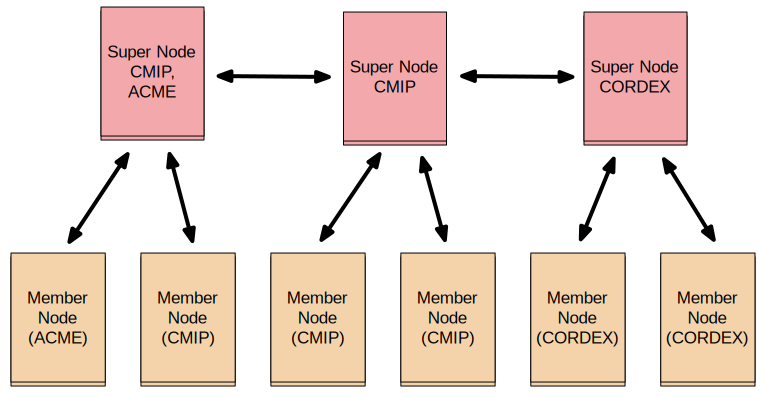
\includegraphics[scale=0.35]{ESG-node-org.pdf}
\end{center}
\end{frame}

\section{Node Manager components}
\begin{frame}{Node Manager components}
\begin{itemize}
\item \textbf{Apache ZooKeeper}, to take care of group management (project), leader election for supernode management etc
\item \textbf{ESGF Node Manager API}, to serve as a wrapper, for ZooKeeper and modify node's availability to be considered for use as supernode etc.
\item \textbf{Metric collector}: query member nodes and aggregate them (supernodes)
\item \textbf{Self-check component}: run sanity checks on self.
\item \textbf{Messaging component}: alert notifications for local admins when services fail.
\item \textbf{Admin console (local node)}: submit membership requests, CSRs, volunteer for supernode role etc
\item \textbf{Admin console (supernode admin mode)}: sign CSRs, manage membership and volunteering requests etc. 
\end{itemize}
\end{frame}

\section{Node Manager component diagram}
\begin{frame}{Node Manager component diagram}
\begin{center}
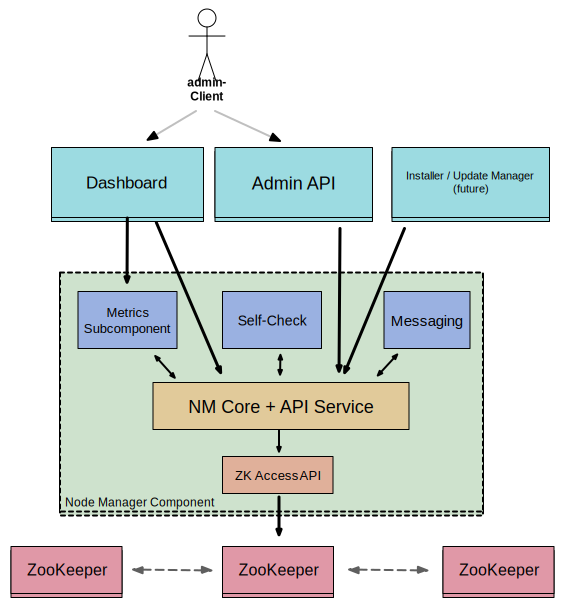
\includegraphics[scale=0.3]{NM-design.pdf}
\end{center}
\end{frame}

\section{Node Manager design considerations}
\begin{frame}{Node Manager design considerations}
\begin{itemize}
\item Security: factor for both user/machine executed elevated privilege operations.
\item Design to guard against spoofing of membernodes/supernodes etc.
\end{itemize}
\end{frame}


\end{document}
